%%%%%%%%%%%%%%%%%%%%%%%%%%%%%%%%%%%%%%%%%%%%
\section{Extras}


%%%%%%%%%%%%%%%%%%%%%%%%%%%%%%%%%%%%%%%%%%%%
\subsection{Ultrasound Needle Tracking}

{
\paper{
\textbf{Xia et. al., 2017} in Scientific Reports DOI:10.1038/s41598-017-03886-4; 
\textbf{Xia et. al., 2016} in MICCAI DOI:10.1007/978-3-319-46720-741
}

\begin{frame}{Ultrasound needle tracking}

\begin{columns}

\begin{column}{.6\linewidth}
	\begin{figure}
        \centering
        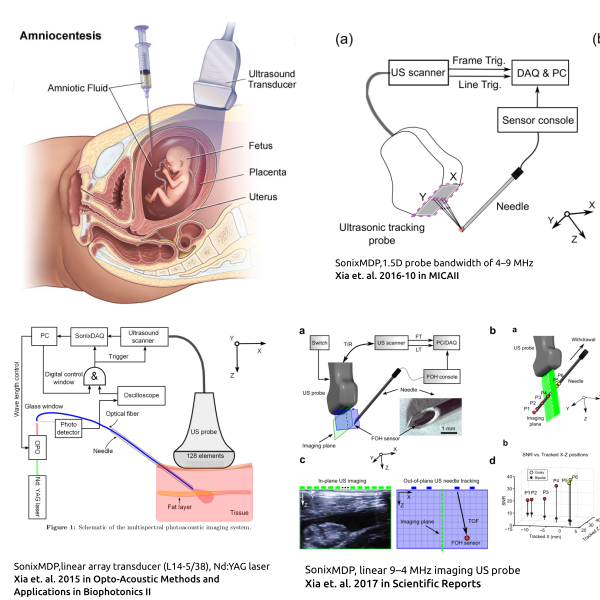
\includegraphics[scale=0.4]{./figs/unt/versions/drawing-v00}
        %\caption{}
      \end{figure}
\end{column}

\begin{column}{.4\linewidth}
	\textbf{Challenges}
        \begin{itemize}
         %\item To see the needle, the ultrasound probe needs to be moved.
	 \item In-plane and out-plane needle tracking
	 \item Needle manipulation is impacted by the experience of the clinitians
	 \item The anatomical view changes.
        \end{itemize}	
\end{column}



\end{columns}

\end{frame}
}



%%%%%%%%%%%%%%%%%%%%%%%%%%%%%%%%%%%%%%%%%%%%
\subsection{Vibro-Tactile Stimulator for Dystonia Research}

%%%%%%%%%%%%%%%%%%%%%%%%%%%%%%%%%%%%%%%%%%%%%%%%%%%%%%%%
{
\paper{MSc. report of Alexander Mitton in collaboration Christos Bergeles, Verity McClelland and Alan Worley}
\begin{frame}{Vibro-Tactile Stimulator for Dystonia Research}

      \begin{figure}
        \centering
        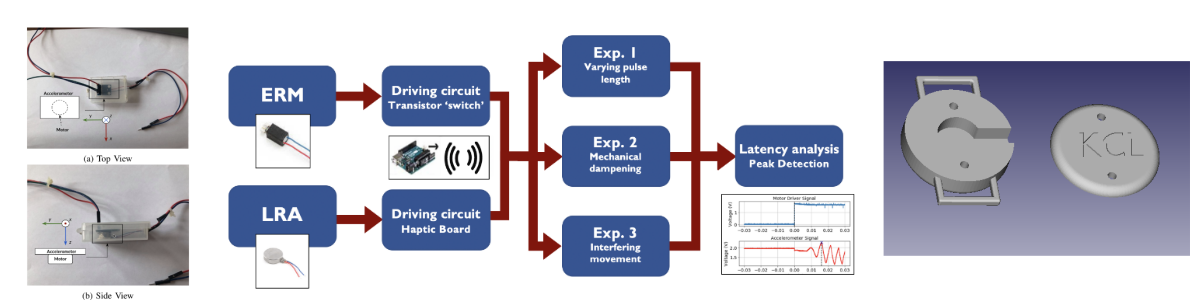
\includegraphics[width=0.99\textwidth]{./figs/event-detection/versions/drawing-v00.png}
        %\caption{}
      \end{figure}

\end{frame}
}




%%%%%%%%%%%%%%%%%%%%%%%%%%%%%%%%%%%%%%%%%%%%
\subsection{free-corTeX: a free CI framework for open scientific communication}
{
\paper{\textbf{Xochicale 2020} in Conf. of Reproducibility, Replicability and Trust in Science \faGithub github.com/mxochicale/rrts2020}

\begin{frame}{
free-corTeX: a free CI framework for open scientific communication
}

      \begin{figure}
        \centering
        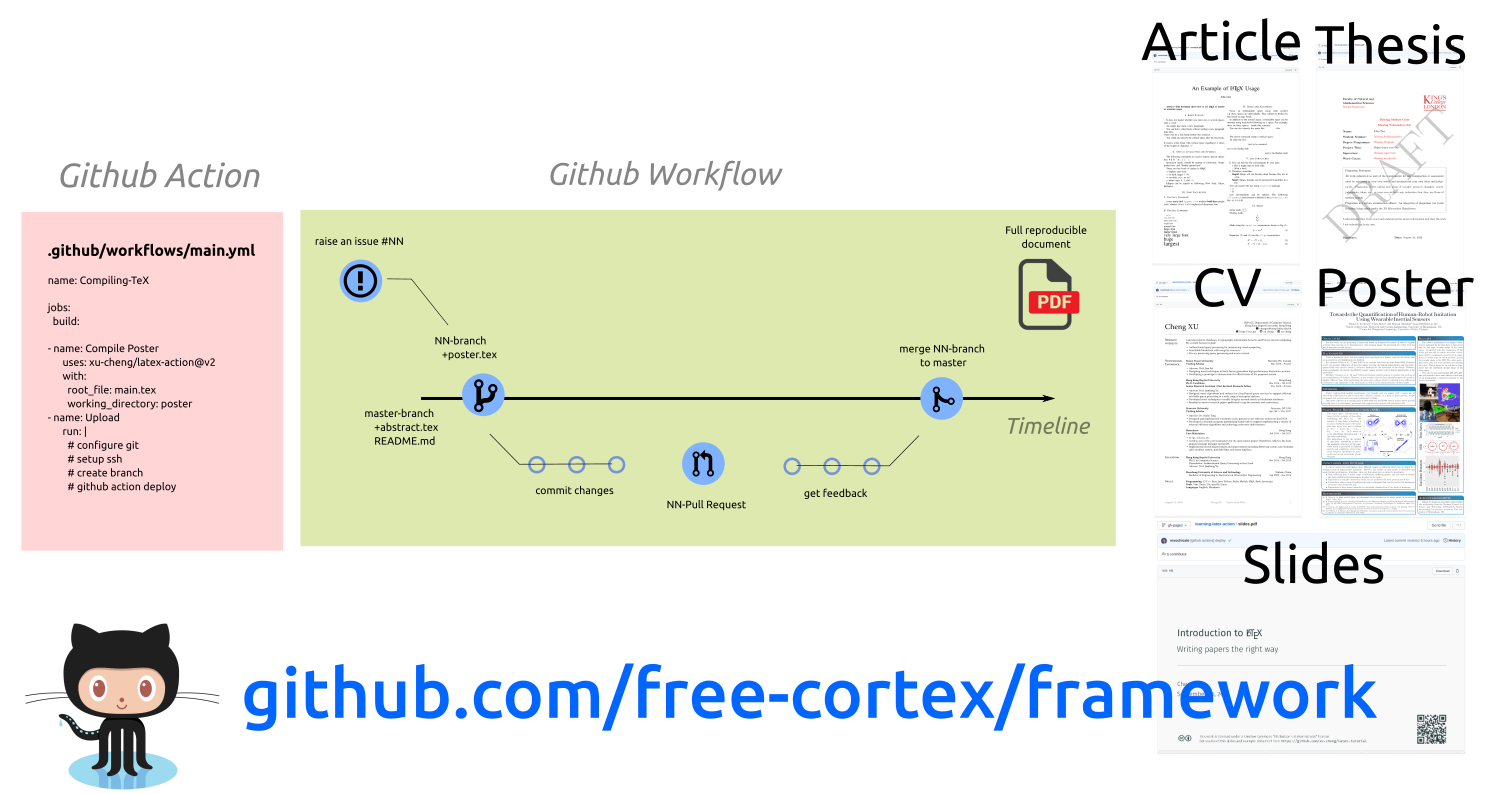
\includegraphics[width=0.95\textwidth]{./figs/free-cortex/versions/drawing-v00.png}
        %\caption{}
      \end{figure}

\end{frame}
}


